\chapter{Marketing Analytics}\label{ch:5}

\begin{remark}{Outline}
In this chapter, we present two different marketing real-world example-dependent 
cost-sensitive problems, namely, churn modeling and direct marketing. Both problems deal 
with identifying those customers with certain characteristic with the objective to maximize the 
results of the different CRM strategies.
First, we introduce the churn modeling problem and present the proposed financial evaluation 
measure for a churn campaign in Section \ref{sec:5:churn}. Lastly in Section 
\ref{sec:5:directmarketing}, the direct marketing problem is presented including the proposed 
example-dependent cost-sensitive cost matrix for evaluating this problem.
\end{remark}


\section{Churn modeling}
\label{sec:5:churn}

Customer churn predictive modeling deals with predicting the probability of a customer defecting 
using historical, behavioral and socio-economical information. This tool is of great benefit to 
subscription based companies allowing them to maximize the results of retention campaigns. The 
problem of churn predictive modeling has been widely studied by the data mining and machine learning
communities. It is usually tackled by using classification algorithms in order to learn the 
different patterns of both the churners and non-churners. Nevertheless, current state-of-the-art 
classification algorithms are not well aligned with commercial goals, in the sense that, the models 
miss to include the real financial costs and benefits during the training and evaluation phases. In 
the case of churn, evaluating a model based on a traditional measure such as accuracy or predictive 
power, does not yield to the best results when measured by the actual financial cost, i.e., 
investment per subscriber on a loyalty campaign and the financial impact of failing to detect a 
real churner versus wrongly predicting a non-churner as a churner.

In this section, we propose a cost-sensitive framework for customer churn predictive 
modeling. First, in Section \ref{sec:5:1:intro}, we introduce 
the problem of chrun modeling. Then in Section \ref{sec:5:1:evaluation}, we present a financial 
based measure for evaluating the effectiveness of a churn campaign taking into account the 
available 
portfolio of offers, their individual financial cost and probability of offer acceptance depending 
on the customer profile. Finally, in Section~\ref{sec:5:1:data}, we describe the real-world churn 
modeling dataset that will be used during the experiments.


\subsection{Flow analysis of a churn campaign}
\label{sec:5:1:intro}

The two main objectives of subscription-based companies are to  acquire new subscribers and 
retain those they already have, mainly because profits are directly linked with the number of 
subscribers.  In order to maximize the profit, companies must increase the customer base by 
incrementing sales  while decreasing the number of churners. Furthermore, it is common knowledge 
that retaining a  customer is about five times less expensive than acquiring a new one 
\citep{Farris2010}, this creates  pressure to have better and more effective churn campaigns.

A typical churn campaign consists in identifying from the current customer base which ones are 
more likely to leave the company, and make an offer in order to avoid that behavior.
With this in mind the companies use intelligence to create and improve retention and collection
strategies. In the first case, this usually implies an offer that can be either a discount or a 
free upgrade during certain span of time. In both cases the company has to 	assume a cost for that 
offer, therefore, accurate prediction of the churners becomes important. The logic of this flow is 
shown in \figurename{ \ref{fig:ch5:1}}.

The churn campaign process starts with the sales that every month increase the customer 
base, however, monthly there is a group of customers that decide to leave the company for many 
reasons. Then the objective of a churn model is to identify those customers before they take the 
decision of defecting.

Using a churn model, those customers more likely to leave are predicted as churners and 
an offer is made in order to retain them. However, it is known that not all customers will accept 
the offer, in the case when a customer is planning to defect, it is possible that the offer is not 
good enough to retain him or that the reason for defecting can not be influenced by an offer.
Using historical information, it is estimated that a customer will accept the offer with 
probability $\gamma$.
On the other hand, there is the case in which the churn model misclassified a non-churner as 
churner, also known as false positives, in that case the customer will always accept the offer that 
means and additional cost to the company since those misclassified customers do not have the 
intentions of leaving.

  \begin{figure}[t]
    \centering
    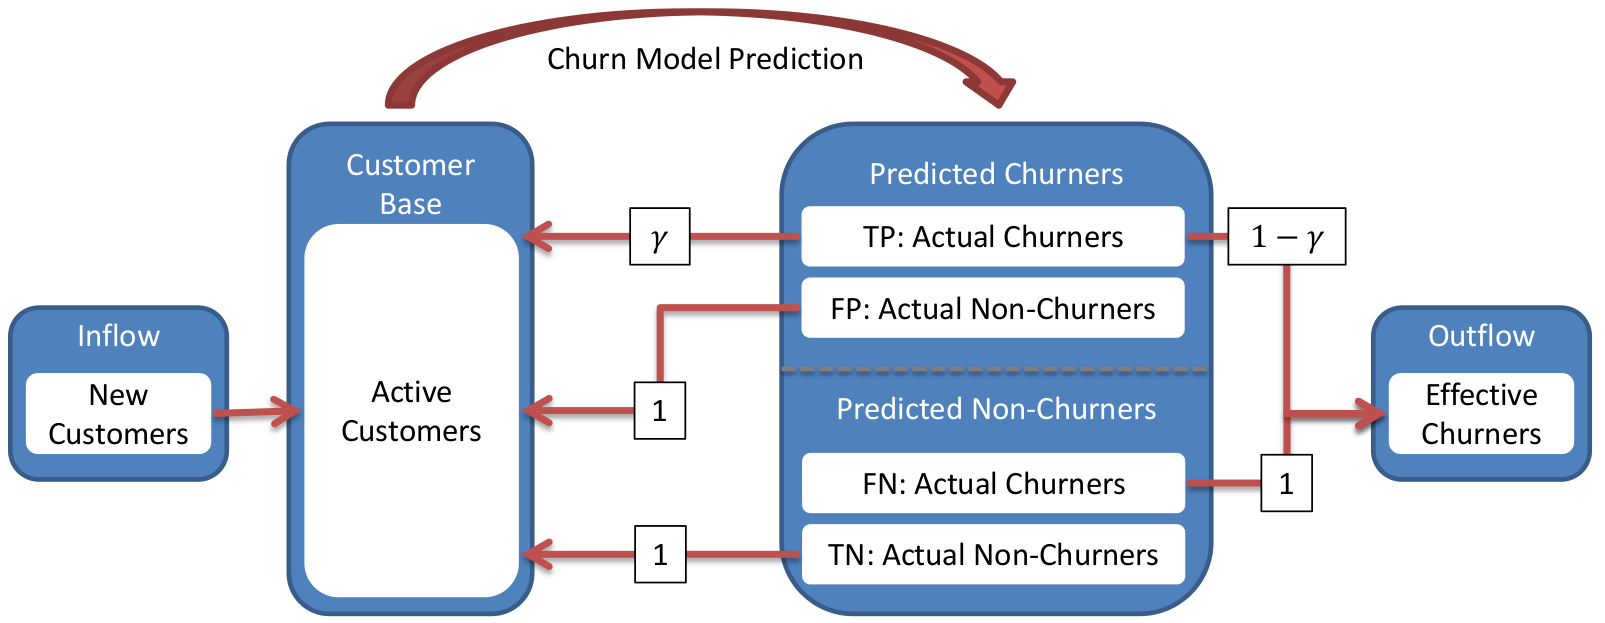
\includegraphics[width=11.5cm]{ch5_fig1}   %CHANGE TO 12cm
    \caption{Flow analysis of a churn campaign \citep{Verbraken2012}}
    \label{fig:ch5:1}
  \end{figure}
  
In the case were the churn model predicts customers as non-churners, there is also the possibility 
of a misclassification, in this case an actual churner is predicted as non-churner, since 
these customers do not receive an offer and they will leave the company, these cases are known as 
false negatives. Lastly, there is the case were the customers are actually non-churners, then 
there is no need to make a retention offer to these customers since they will continue to be part 
of the customer base.

It can be seen that a churn campaign (or churn model) has three main points. First, avoid false 
positives since there is a financial cost of making an offer where it is not needed. Second, find 
the right offer to give to those customers identified as churners. And lastly, to decrease 
the number of false negatives.

From a machine learning perspective, a churn model is a classification algorithm.
In the sense that using historical information, a prediction of which current customers 
are more likely to defect, is made. This model is normally created using one of a number of 
well established algorithms (Logistic regression, neural networks, random forests, among 
others) \citep{Ngai2009,KhakAbi2010}. Then, the model is evaluated using measures such as 
misclassification error, receiver operating characteristic ($ROC$),  Kolmogorov-Smirnov ($KS$) 
or \mbox{$F_1Score$} statistics \citep{Verbeke2012}. 
However, these measures may not be the most appropriate evaluation criteria when  
evaluating a churn model, because they tacitly assume that misclassification errors carry the 
same cost, similarly with the correct classified examples. This assumption does not hold in many 
real-world applications such as churn modeling, since  when misidentifying a churner the financial 
losses are quite different than when misclassifying a non-churner as churner \citep{Glady2009}. 
Furthermore, the accuracy measure also assumes that the class distribution 
among examples is constant and balanced \citep{Provost1998}, and typically the distributions of a 
churn data set are skewed \citep{Verbeke2012}.
	
In the next section, we propose a new financial based measure for evaluating the effectiveness of 
a voluntary churn campaign taking into account the available portfolio of offers, their 
individual 	financial cost and probability of acceptance depending on the customer profile. 


\subsection{Propose evaluation measure of a churn campaign}
\label{sec:5:1:evaluation}
	
Different studies have proposed measures to deal with these cost-sensitivity related to
evaluating a churn model. In \citep{Neslin2006}, a profit-based measure was proposed by starting 
with the confusion matrix and multiplying it with the expected profit of each case.

\begin{align}\label{eq:5:profit1}
 Profit_1 = (TP+FP)\bigg[ & \left(\gamma CLV + C_o(1-\gamma)(-C_a)\right)\pi_1\gamma \nonumber \\
 & -C_o-C_a\bigg]-N\cdot C_a,
\end{align}
with $C_a$ being the fixed administrative cost of running the campaign, $C_o$ the average 
cost of the retention offer, $C_a$ the cost of contacting the customer, $\pi_1$ the prior churn rate 
and $CLV$ the average customer lifetime value or the present value of the expected profit that a 
customer will generate. Moreover, as discussed in \citep{Verbraken2013}, if the average instead of 
the total profit is considered and the fixed cost $N\cdot C_a$ is discarded since it is irrelevant 
for the classifier selection, the profit can be expressed as:
\begin{align}\label{eq:5:profit2}
 Profit_2 = &TP\left(\gamma(CLV-C_o-C_a)+(1-\gamma)C_a \right) \nonumber \\
 &+FP(-C_o-C_a).
\end{align}

Nevertheless, equations (\ref{eq:5:profit1}) and (\ref{eq:5:profit2}) assume that every customer 
has the same $CLV$ and $C_o$, whereas this is not true in practice. In fact, different customers 
have a very different $CLV$, and not all offers can be made to every customer, neither do they have 
the same impact across customers. In order to obtain a more business oriented measure, we first 
analyze the financial impact of the different decisions, i.e., false positives, false negatives, 
true positives and true negatives, for each customer.	

\begin{figure}[t]
  \centering
  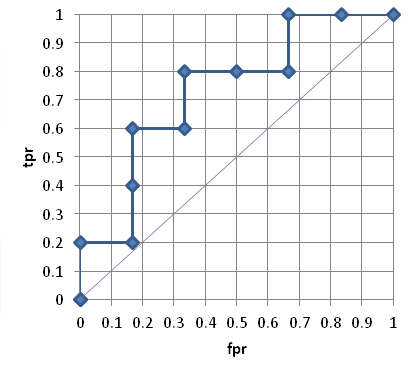
\includegraphics[width=12cm]{ch5_fig2}
  \caption{Financial impact of the different decisions, i.e., False positives, false negatives, 
  true 	positives and true negatives}
	\label{fig:ch5:2}
\end{figure}

In \figurename{ \ref{fig:ch5:2}}, the financial impact of a churn model is shown. Note than we take 
into account the costs and not the profit in each case.
When a customer is predicted to be a churner, an offer is made with the objective of avoiding 
the customer defecting. However, if a customer is actually a churner, he may or not accept the 
offer with a probability $\gamma_i$. If the customer accepts the offer, the financial impact is 
equal to the cost of the offer ($C_{o_i}$) plus the administrative cost of contacting the 
customer ($C_a$). On the other hand, if the customer declines the offer, the cost is the 
expected 	income that the clients would otherwise generate, also called customer lifetime value 
($CLV_i$), 	plus $C_a$. Lastly, if the customer is not actually a churner, he will be happy to 
accept the 	offer and the cost will be $C_{o_i}$ plus $C_a$.
	
In the case that the customer is predicted as non-churner, there are two possible outcomes. 
Either the customer is not a churner, then the cost is zero, or the customer is a churner and the 
cost is $CLV_i$. 


  \begin{table}[b]
	  \centering
	  \footnotesize
     \begin{tabular}{c|c|c}
        \multicolumn{3}{c}{}\\
			\multicolumn{1}{c|}{}  & Actual Positive& Actual Negative \\
			\multicolumn{1}{c|}{} & $y_i=1$& $y_i=0$ \\
			\hline
			Predicted Positive 		& $C_{TP_i}=\gamma_iC_{o_i}$ & 
\multirow{2}{*}{$C_{FP_i}=C_{o_i}+C_a$}\\
%       Predicted Positive    & \multirow{ 
% 2}{*}{$C_{TP_i}=\gamma_iC_{o_i}+(1-\gamma_i)(CLV_i+C_a)$} & 
% \multirow{2}{*}{$C_{FP_i}=C_{o_i}+C_a$}\\
			$c_i=1$ & $+(1-\gamma_i)(CLV_i+C_a)$ &\\
			\hline
			Predicted Negative  	& \multirow{ 2}{*}{$C_{FN_i}=CLV_i$} & \multirow{ 
			2}{*}{$C_{TN_i}=0$} \\
			$c_i=0$ & &\\
			%\hline
		\end{tabular}
		\caption{Proposed churn modeling example-dependent cost matrix}
    \label{tab:ch5:1}
  \end{table}

The different costs are summarized in \tablename{ \ref{tab:ch5:1}}.	Then using the cost 
matrix, and the example-dependent cost-sensitive framework as described in Section 
\ref{sec:3:csmeasures}, an example-dependent cost statistic is calculated as:

\begin{align}
  Cost_i &= y_i(c_i C_{TP_i} + (1-c_i)C_{FN_i})& \nonumber \\
         &  + (1-y_i)(c_i C_{FP_i} + (1-c_i)C_{TN_i})& \nonumber \\
%          &=y_i(c_i (\gamma_iC_{o_i}+(1-\gamma_i)(CLV_i+C_a))& \nonumber \\
%          & + (1-c_i)CLV_i)& \nonumber \\
%          & +  (1-y_i)(c_i (C_{o_i}+C_a) + (1-c_i)(0)) &\nonumber \\
         &= y_i(c_i\left(\gamma_i(C_{o_i}-CLV_i-C_a)-C_{o_i}\right)+CLV_i)&\nonumber \\
         & +c_i(C_{o_i}+C_a),&
	\end{align}
leading to a total cost of:
\begin{equation}
    Cost = \sum_{i=1}^N Cost_i.
\end{equation}
Furthermore, using (\ref{eq:3:savings}), the savings are calculated as:
\begin{equation}
  Savings = \frac{Cost_l - Cost}{Cost_l},
\end{equation} 
In almost all cases the costless class ($Cost_l$) will be the negative class, as typically the 
distribution of a churn dataset is skewed towards the non-churners \citep{Verbeke2012}. Given that 
$Cost_l$ can be expressed as $Cost(f_0)$, or simply $Cost$ with $c_i=0$ $\forall i$:
\begin{equation}
 Cost_l = \sum_{i=1}^{N} y_i CLV_i.
\end{equation}
This is consistent with the notion that if no model is used, the total cost would be the 
sum of the customer lifetime values of the actual churners, which gives the insight 
that the $Savings$ measure consists in comparing the financial impact of the campaign of using a 
classification model against not using a model at all.


\subsubsection{Customer lifetime value}

Lastly, one of the key values to calculate the $Savings$ is the customer lifetime value. Within 
marketing there exists a common misconception between customer profitability and customer lifetime 
value. The two terms are usually used in an interchangeable way, 
creating confusion of what the actual objective of a churn modeling campaign should be. Several 
studies have proposed models providing a unique definition of both terms 
\citep{Neslin2006,Pfeifer2004,Milne1999a,VanRaaij2003}. Customer 
profitability indicates the difference between the income and the cost 
generated by a customer $i$ during a financial period $t$. It is defined as: 
\begin{equation}
	CP_{i,t} = \mu  \cdot s_{i,t},
\end{equation}
where  $s_{i,t}$ refers to the consumption of customer $i$ during time period $t$, and $\mu$ refers 
to the average marginal profit by unit product usage.  

Moreover, we are interested to see what is the expected income that a particular customer will 
generate in the future, in other words, calculating the expected sum of 
discount future earnings \citep{Neslin2006}. Therefore, the $CLV_i$ is defined as:
\begin{equation}
	CLV_i = \sum_{t=1}^T\frac{\mu \cdot s_{i,t}}{(1+r)^t},
\end{equation}
where $r$ is the discount rate, and $T$ the number of time period.
Typically $T$ should be considered large enough since without prior 
knowledge a customer is expected to keep being a customer for the foreseeable future. In practice 
$T$ is set up to be infinity~\citep{Glady2009}. Also, for simplicity, it can be assumed that 
$s_{i,t+1}=s_{i,t}\cdot (1+g)$ $\forall {i,t}$, which means that there is a constant growth $g$ in 
the customer consumption. Given that, the customer lifetime value can be re-written as
\begin{equation}
 CLV_i = \sum_{t=1}^\infty\frac{ (1+g)^t}{(1+r)^t}\cdot \mu\cdot s_{i,1},
\end{equation}
which in the case of $g<r$, this is a geometric series and can be expressed as
\begin{equation}
 CLV_i = \frac{\mu\cdot s_{i,1}}{(r-g)}.
\end{equation}


\subsection{Churn modeling database}
\label{sec:5:1:data}

For our experiments we use a dataset provided by a TV cable provider. 
The dataset consists of active customers during the first semester of 2014. 	
The total dataset contains 9,410 individual registries, each one with 45 attributes, 
including a churn label indicating whenever a customer is a churner.
This label was created internally in the company, and can be regarded as highly accurate. 
In the dataset only 455 customers are churners, leading to a churn ratio of 4.83\%.
	
\subsubsection{Offer acceptance calculation}

In practice companies have a set of offers to make to a customer as part of the retention 
campaign. They vary from discounts to upgrades, among others. In the particular case of a TV cable 
provider, the offers include adding a new set of channels, changing the TV receiver to one with new 
technology (i.e., high definition, video recording, 4K),  or to offer a discount on the monthly 
bill. Unsurprisingly, not all offers apply to all clients. For instance, a customer that already 
has all  the channels can not be offered a new set of channels. Moreover, an offer usually means an 
additional cost to the company and not all offers have the same cost or the same impact in 
reducing churn.

Taking into account the cost and the implication of the offers, the problem can be 
summarized in making each customer the offer that will maximize the acceptance rate and more 
importantly reduce the overall cost. 

\begin{figure}[t!]
  \centering
   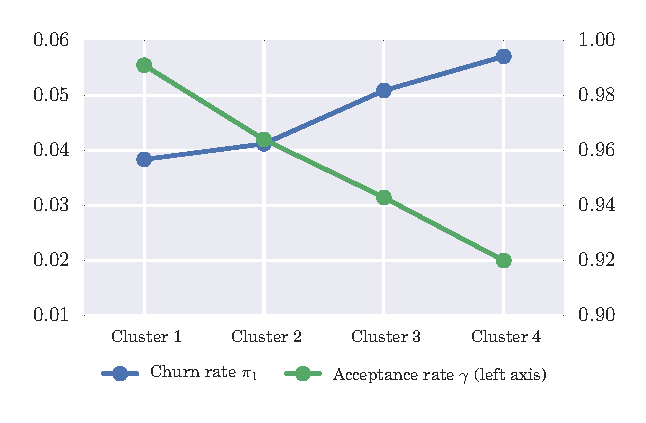
\includegraphics[width=10cm]{ch5_fig3}
  \caption{Acceptance rate ($\gamma$) of the best offer for each customer profile. As expected, 
	the higher the churn rate the lower the acceptance rate, as it is more difficult to make a 
	good offer to a customer which is more likely to defect. }
  \label{fig:ch5:3}
\end{figure}

In order to calculate the acceptance probability $\gamma_i$ a champion-challenger process was made. 
First, the customers were grouped into clusters according to their behavioral and socio-economical 
characteristics. In particular the K-means algorithm was used \citep{Marslan2009}.
Then for a period of two months, randomly selected offers were made to the customers and their 
response was evaluated. Unfortunately, for confidentiality reasons we can not describe the 
different clusters, or the actual offer made to each customer. Nevertheless, in 
\figurename{~\ref{fig:ch5:3}}, the average churn rate and acceptance rate $\gamma_i$ per cluster is 
shown. As expected, the higher the churn rate the lower the acceptance rate, as it is more difficult 
to make a good offer to a customer that is more likely to defect.


\section{Direct marketing}
\label{sec:5:directmarketing}

In direct marketing the objective is to classify those customers who are more likely to have a 
certain response to a marketing campaign \citep{Ngai2009}. We used a direct marketing dataset 
\citep{Moro2011} available on the UCI machine learning repository \citep{UCI2013}. The dataset 
contains 45,000 clients of a Portuguese bank who were contacted by phone between March 2008 and 
October 2010 and received an offer to open a long-term deposit account with attractive interest 
rates.  The dataset contains features such as age, job, marital status, education, average yearly 
balance and current loan status and the label indicating whether or not the client accepted 
the offer.

This problem is example-dependent cost sensitive, since there are different costs of false 
positives and false negatives. Specifically, in direct marketing, false positives have the cost 
of contacting the client, and false negatives have the cost due to the loss of income by failing 
to contact a client that otherwise would have opened a long-term deposit. 
  
\begin{table}[b]
  \centering
  \footnotesize
  \begin{tabular}{c|c|c}
    \multicolumn{1}{c|}{}  & Actual Positive& Actual Negative \\
    \multicolumn{1}{c|}{} & $y_i=1$& $y_i=0$ \\
    \hline
    Predicted Positive    & \multirow{ 2}{*}{$C_{TP_i}=C_a$} & \multirow{ 2}{*}{$C_{FP_i}=C_a$} 
    \\
    $c_i=1$ & &\\
    \hline
    Predicted Negative    & \multirow{ 2}{*}{$C_{FN_i}=Int_i$} & \multirow{ 2}{*}{$C_{TN_i}=0$} 
    \\
    $c_i=0$ & &\\
    %\hline
  \end{tabular}
  \caption{Direct marketing example-dependent cost matrix}
  \label{tab:5:d_mat}
\end{table}

We propose a direct marketing example-dependent cost matrix as shown in \mbox{\tablename{ 
\ref{tab:5:d_mat}}}. Where $C_a$ is the administrative cost of contacting the client, as is credit 
card fraud,  and $Int_i$ is the expected income when a client opens a long-term deposit. This last 
term is defined as the long-term deposit amount times the interest rate spread.
 
In order to estimate $Int_i$, first the long-term deposit amount is assumed to be a 20\% of the 
average yearly balance, and lastly, the interest rate spread is estimated to be 2.463\%,  which 
is the average between 2008 and 2010 of the retail banking sector in Portugal as reported by the 
Portuguese central bank. Given that, the $Int_i$ is equal to $\left( balance * 20\% \right) * 
2.463\%$.


\section{Summary of the datasets}

In this section we present the different marketing datasets. 
For each dataset we used a pre-define cost matrix as shown in Section~\ref{sec:5:churn} and 
Section~\ref{sec:5:directmarketing}. Moreover,  the datasets are split in training, validation 
and testing, each one containing 50\%, 25\% and 25\% of the examples, respectively. Afterwards, 
an under-sampling of the positive examples is made, and we perform the 
cost-proportionate rejection-sampling and cost proportionate over-sampling procedures, as described 
in Section~\ref{sec:3:costsampling}. \tablename{~\ref{tab:5:databases}}, 
summarizes the different datasets. 

\begin{table}%[ht!]
  \centering
  \footnotesize
  \begin{tabular}{l l c c c } %sum 7.7
    \hline
    \textbf{Database}& \textbf{Set}&  $N$ & $\pi_1$ & Cost (Euros) \\
    \hline
    Churn&Total&9,410&4.83&580,884\\
    Modeling&Training ($t$)&3,758&5.05&244,542\\
    &Under-sampled ($u$) &374&50.80&244,542\\
    &Rejection-sampled ($r$)&428&41.35&431,428\\
    &Over-sampled ($o$) &5,767&31.24&2,350,285\\
    &Validation&2,824&4.77&174,171\\
    &Testing&2,825&4.42&162,171\\
    \hline
    Direct &Total&37,931&12.62&59,507\\
    Marketing&Training ($t$)&15,346&12.55&24,304\\
    &Under-sampled ($u$)&3,806&50.60&24,304\\
    &Rejection-sampled ($r$)&1,644&52.43&20,621\\
    &Over-sampled ($o$)&22,625&40.69&207,978\\
    &Validation&11,354&12.30&16,154\\
    &Testing&11,231&13.04&19,048\\
    \hline
  \end{tabular}
  \caption{Summary of the marketing datasets, where $N$ is the number of examples and $\pi_1$ is 
  the percentage of positive examples.}
  \label{tab:5:databases}
\end{table}
 
%  \makeatletter
% \setlength{\@fptop}{0pt}
% \makeatother